\chapter{Design}\label{chDesign}
	
	\section{The Architecture}
	This section gives a high level overview of the architecture of the software by introducing its main building blocks and the main modules they interact with. 
	%Image \ref{fig:architecture} shows the building blocks of the developed components and the modules
  
	Image \ref{fig:architecture} on the left side contains the vision module, composed by the sub-modules \emph{Server} and \emph{Visual Operations}, and, on the right, \mbox{Lisp} interpreters that run \mbox{ACT-R} models.
	%On the right there are \mbox{ACT-R} models, executed by \mbox{Lisp} interpreters.
	The two parts communicate to each other thanks to a \mbox{client-server} communication mechanism based on \mbox{TCP/IP} protocol in which the \mbox{Lisp} interpreter represents the client and the visual module the server.
	
	\begin{figure}[h]
	  \begin{center} 
	    \fbox{	
	       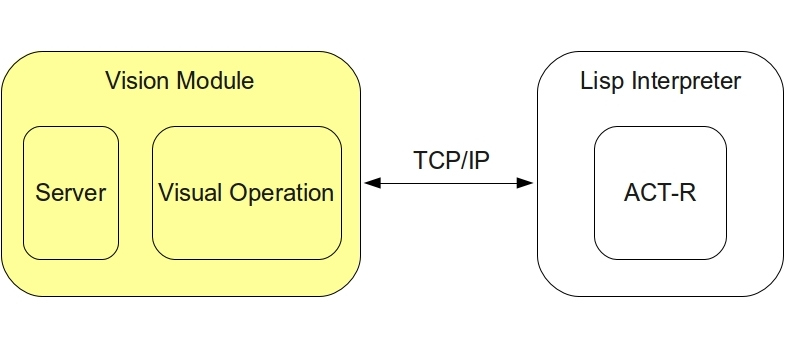
\includegraphics[width=\textwidth*\real{0.9}]{images/ch_05/architecture.jpg}
	    }
	  \end{center} 
	  \caption{\textit{High level scheme of the architecture}}  
	  \label{fig:architecture}
 	\end{figure}


	\mbox{ACT-R} part is not discussed in this work but is fundamental for the choices about the communication protocol.
	This document focuses on the \emph{Vision Module}, whose main operations are extracting features from the input data and sending them to the models in a way that can be understood by the cognitive architecture. 
	These functions are realized by the two sub-modules contained in Vision Module.
	%The vision module does not take part in the cognitive reasoning; rather it extracts useful information that can be used by the model in its reasoning activity.

	\section{Processes}
	Figure \ref{fig:processes} represents a scheme of processes and threads that compose the architecture.
	As shown in the picture, the \mbox{Lisp} interpreter and the visual module run on two separated processes. 
	The processes are independent and their management is left to the operative system.

	The design on the communication protocol is such that the two processes can be run only on the same computer. 
	The images to be processed, in fact, at the moment are not sent as messages from the client to the server but are stored on the computer which runs both the processes.
	Anyway, it is enough to modify the message exchange by adding a message sent from the client to the server encapsulating the image data in order to run them on two different computers.
	
	\begin{figure}[h]
	  \begin{center} 
	    \fbox{	
	       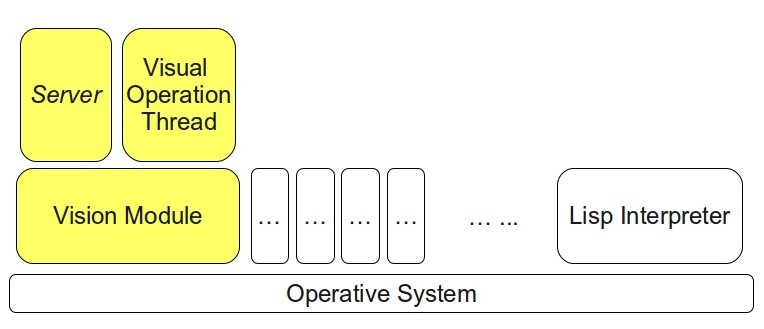
\includegraphics[width=\textwidth*\real{0.9}]{images/ch_05/processes.jpg}
	    }
	  \end{center} 
	  \caption{\textit{High level scheme of the architecture}}  
	  \label{fig:processes}
 	\end{figure}

	
	The Vision Module is composed by two threads: one for the server and the other for the visual processing. 
	The server thread runs in background while the visual operation one is the main thread.
	The problems regarding \mbox{race conditions} are dealt with \emph{semaphores}; all the other issues are automatically managed by the \emph{Boost} library.
	The thread organization of \mbox{ACT-R} is not discussed in this work.	


	\section{Communication}
	In order to exchange information between each other, \mbox{ACT-R} and the developed module use a synchronous \emph{client-server} communication mechanism based on \mbox{TCP}. 
	\mbox{ACT-R} models represent the clients, the developed software the server. 
	The format used for the messages is \mbox{JSON}.  		

	The client-server approach has been chosen because it is standardized and is supported by the interpreters that run \mbox{ACT-R}. 
	Moreover, the time spent for coding and decoding the message is negligible if compared to the time needed for the image processing.
	Finally, the possibility of using shared resources and the transparency offered by the mechanism ensure very high flexibility and scalability.
	

\begin{comment}
	The client-server approach has been chosen because it is standardized and is supported by the interpreters that run \mbox{ACT-R}. 
	In addition, the possibility of using shared resources and the transparency offered by the mechanism ensure very high flexibility and scalability.
	The con of this method is the overhead introduced for the inter process communication. In fact, it needs an intermediate format of messages and instruments for coding and decoding data.
	In this case, anyway, the time needed to perform these operations is negligible if compared to the time needed for the image processing.
\end{comment}

	Another solution analyzed for the communication between \mbox{ACT-R} and the Visual Module is compiling the Visual Module as a static library and then loading it directly in the \mbox{Lisp} interpreter.
	The latter is able to call the static functions thanks to \emph{foreign functions}.
	%The calls to the static library are then called thanks to a wrapper and 
	In this way, the communication is more efficient because all the overhead introduced due to the inter process communication is avoided. 
	This method, though, is not maintainable. 
	In fact, every \mbox{Lisp} interpreter has a different method of calling foreign functions~\cite{SWIGDoc}. 
	As consequence of this, every time the interpreter is changed, the interface of the visual module must be re-written.
 	At design time it has been decided to prefer maintainability to an irrelevant improvement of the performances, thus the client-server has been preferred to this solution.

	TCP has been preferred to \mbox{UDP} mainly because of the reliability guaranteed by that protocol. 
	Secondly, the bi-directionality of the communication and the small quantity of data exchanged make it more suitable for the purpose.

	The communication is synchronous. 
	The client, once having sent the request, stays pending until it receives the response. 
	This choice is coherent with the application domain: as the software module acts like a vision system for the cognitive architecture, it makes sense that the model does not continue the reasoning until the available visual information is received.

	The \mbox{Lisp} interpreter which runs \mbox{ACT-R} models is the client, while the developed software is the server.  	
	When a model needs to acquire information about an image, it connects to the server. 
	Once connected, it can encode and send a request to the server. 
	After the server has received and decoded successfully the request, it processes the input data. When the visual information are ready to be sent, the server encodes them and send them back to the client. 
	After this, the message is decoded and its content is translated in chunks and then delivered to the model, that uses it for the cognitive reasoning.

	All the messages exchanged between client and server are encoded in \mbox{JSON}. 
	Appendix \ref{appB} contains an example of the messages.
%		In the next paragraph will be described more in detail how the data are encoded.


	\section{Vision Operation Module}
	The vision operation module is composed of three main parts, one for processing images and videos, one for containing the hierarchy of the objects recognized during such processing and one containing the exception classes and the utility functions used by all the other components.

\begin{comment}
	The vision module is composed of four main parts, one for processing images and videos, one for containing the hierarchy of the objects recognized during such processing, one for the communication with the model and one containing all the utility functions used by all the other components.
\end{comment}	

	%\todo{change picture}
	\begin{figure}[h]
	  \begin{center} 
	    \fbox{	
	       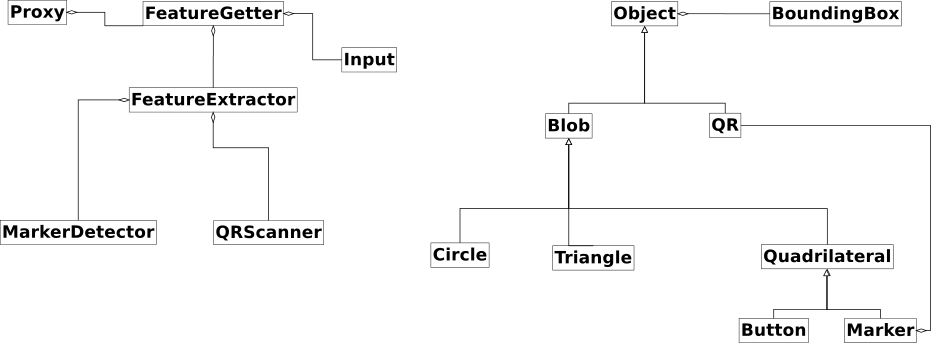
\includegraphics[scale=0.55]{images/ch_05/progettazione_overview.png}
	    }
	  \end{center} 
	  \caption{\textit{Class diagram illustrating a high level overview of the vision operation module}}  
	  \label{fig:classOverview}
 	\end{figure}

	%\todo{change this part}
	Image \ref{fig:classOverview} shows a class diagram which describes two of the parts that compose the software. 
	The part dedicated to the processing of images and videos is located on the left and is composed by the classes \emph{Proxy}, \emph{FeatureGetter}, \emph{FeatureExtractor}, \emph{Input}, \emph{MarkerDetector} and \emph{QRScanner}.
	The object hierarchy, which is shown on the right, contains the classes \emph{Object}, \emph{BoundingBox}, \emph{Blob}, \emph{QR}, \emph{Circle}, \emph{Triangle}, \emph{Quadrilateral}, \emph{Button} and \emph{Marker}.

	%\todo{change this part}
	The third part is not included in the section because it contains only utility classes and functions. 
	The reader can find a description of that part in appendix \ref{appB}. 

\begin{comment}
	The other part is not included in the design diagrams for different reasons. 
	According to the non-functional requirements, the team planned to try different solutions in order to implement the communication between the software and ACT-R. As different approaches can lead to different architectures, this part has not been designed a priori.
	Regarding the utility part, it depends strongly by the future design and implementation choices and is influenced by the chosen communication technique. These factors make it very instable and volatile. 
	For these reasons and according to the agile development, the team decided not to spend time in planning a fixed structure for it at the beginning.
\end{comment}
	
